\documentclass{sig-alternate}
\usepackage{url}
\usepackage{graphicx}
\usepackage{subfigure}
\usepackage{url}

\begin{document}

\newcommand{\todo}[1]{\textbf{TODO}\footnote{\textbf{TODO:} #1}}


\title{An exploration of the pull-based software development model}
\numberofauthors{3}

\author{
\alignauthor
Georgios Gousios\\
       \affaddr{Delft University of Technology}\\
       \affaddr{Delft, The Netherlands}\\
       \email{G.Gousios@tudelft.nl}
\alignauthor
Martin Pinzger\\
       \affaddr{Delft University of Technology}\\
       \affaddr{Delft, The Netherlands}\\
       \email{M.Pinzger@tudelft.nl}
\alignauthor
Arie van Deursen\\
       \affaddr{Delft University of Technology}\\
       \affaddr{Delft, The Netherlands}\\       
       \email{Arie.vandeursen@tudelft.nl}
}

\maketitle

\begin{abstract}

  The advent of distributed version control systems has led to the development
  of a new paradigm for distributed software development; instead of pushing
  changes to a central repository, developers pull them from other repositories
  and merge them locally. Various code hosting sites, notably Github, have
  tapped on the opportunity to facilitate pull based development by offering
  workflow support tools, such as code reviewing systems and integrated issue
  trackers. In this work, we provide an exploration of how pull-based software
  development works. By quantitatively analysing a hundred projects, we
  identify the factors that affect pull request processing speed and
  create a classifier able of predicting whether pull requests will be accepted
  with 85\% accuracy.  

\end{abstract}

% A category with the (minimum) three required fields
\category{H.4}{Information Systems Applications}{Miscellaneous}
%A category including the fourth, optional field follows...
\category{D.2.8}{Software Engineering}{Metrics}[complexity measures, performance measures]

\terms{Theory}

\keywords{pull-based development, pull request, collaborative development}

\section{Introduction}

%Several code hosting sites, including Github and BitBucket, tapped on the
%opportunity to make the pull-based development model more accessible to
%programmers. A unique characteristic of such sites is that they allow any user
%to fork any public repository. The clone creates a public project that belongs
%to user that cloned it, so the user can modify the repository without being part
%of the development team. What is more important is they automate the selective
%contribution of commits from the clone to the source, through pull requests. As
%mentioned earlier, pull requests are not unique to code hosting sites; in fact,
%the Git software distribution includes the \textsf{git-request-pull} utility
%which provides the same functionality at the command line. Github
%improved\footnote{Not everyone agrees:
%\url{https://github.com/torvalds/linux/pull/17}} this process significantly by
%integrating code reviews, discussions and issues, thus effectively lowering the
%entry barrier for casual contributions. Combined, cloning and pull requests
%create a new development model, where changes are pushed to the project
%maintainers and go through code review by the community before being integrated. 
%


Software development can be distributed across various
dimensions~\cite{Gumm06}; among them, physical distribution distributes
programming tasks across people collaborating remotely, while temporal
distribution distributes tasks to people working in different time zones.
Distribution of development activities has been initially thought to hinder
collaboration~\cite{Herbs99, Batti01}, even though subsequent studies have
shown that it does not pose significant threats to project
quality~\cite{Spine06, Nguye08, Bird09a}. Access to online collaboration tools
such as {\sc vcs} and bug databases have been identified as a necessary
requirement for collaborative software development~\cite{Knuds76,Pilat06,
Catal06}. Moreover, distributed collaboration on software artifacts can be
facilitated through awareness building tools~\cite{Dabbi12, Treud12, Lanza10}. 

Pull-based development is an emerging paradigm for distributed software
development. As more developers appreciate the perceived benefits of isolated
development and branching~\cite{Bird12}, more projects, both closed source and,
especially, open source are being migrated to code hosting sites with support
for pull based development~\cite{Barr12}.

We advocate that pull requests as a distributed development model in general,
and as are implemented by Github in particular, form a new method of
collaboration for distributed software development. The novelty lays on
the decoupling of the development effort from the decision to incorporate
the results of the development in the code base. 
By separating the concerns of building artifacts and incorporating
changes, work is cleanly distributed among a core team which is responsible
to perform the merges and a peripheral team that submits, often occasional,
changes to be considered for merging.

Previous work has identified the processes of collaboration in open source
through patch submission and acceptance~\cite{MOCKU02, Bird07, Weiss08}.  There
are many similarities to the way pull requests work; for example, similar work
team structures emerge (the ``onion'' model~\cite{Crow05}) while the process to
accept a patch goes through a similar assessment process.  What pull requests
bring in addition is process automation and centralization of information.
With pull requests, the code does not have to leave the revision control
system, and therefore it can be versioned across repositories, while authorship
information is effortlessly maintained. Communication is context-specific
(revolving around a single pull request) while .  Moreover, the review
mechanism that Github incorporates has the additional effect of improving
awareness~\cite{Dabbi12}; core developers can access in an efficient way all
information that relates to an application patch/pull request and solicit the
opinions of the community (``crowd-source'') about the merging decision.

The goal of the paper is to analyze the factors that affect the efficiency
of the pull-based software development model. Specifically, the questions we are trying to answer are: 
%Intuitively, a pull
%request based collaboration is effective when the suitability of the pull
%request for a project can be assessed fast. 

\begin{description}

  \item[RQ1] What factors affect the decision to merge a pull request?

  \item[RQ2] What factors affect the time required to process a pull request,
    until it is merged?

\end{description}

Our study is based on data from the Github collaborative development forge, as
made available through the GHTorrent project~\cite{GS12}. Using it, we first
explore the use of pull requests across all projects in Github.  We then examine
82 carefully selected Ruby, Java and Scala projects, (35,466 pull requests), and
identify, using machine learning tools, common factors that affect pull request
lifetime and merging. The results show that pull requests \emph{acceptance}
can be predicted with high accuracy (> 90\%), while it is mostly dependent on
what parts of the system does the pull request affect.  On the other hand, pull
request \emph{merge time} can be predicted with reasonable accuracy (> 70\%),
while it is mostly dependent on the ensuing discussion and the test coverage of
the target project.  Both results can be exploited to assist developers to
submit better pull requests, project managers to prioritize pull requests, while
it opens new opportunities for research, such as building automated tools for
pull request triaging.

This work makes the following concrete contributions:

\begin{itemize}

  \item Descriptive statistics on the use of pull requests in github, demonstrating, e.g., a significant increase in the involvement of external collaborators since the introduction of the github pull request in 2010 

  \item We identify the factors that affect pull request acceptance and
    speed of processing

\end{itemize}


\section{Background}

Since their appearance in 2001, distributed version control systems ({\sc
dvcs}), notably Git, have revolutionized the way distributed software
development is carried out. Driven by pragmatic needs, {\sc dvs}s were designed
from scratch to work as an advanced patch management systems, rather than a
versioned file system, the then dominant version control system ({\sc vcs})
paradigm. In most {\sc dvcs}s, a file is an ordered set of changes, the serial
application of which lead to the current file, and consequently file tree,
state. The changesets can originate from a local filesystem or a remote host;
tools facilitate the acquisition and application of changesets on a local
mirror. The distributed nature of {\sc dvcs}) enables a pull-based development
model, where changes are offered to a project repository through a network of
project forks; it is up to the repository owner to accept or reject the incoming
pull requests.

The development models afforded by {\sc dvcs}s are a superset of 
those in centralized version control environments~\cite{Shiha12,Bird09}. 
With respect to receiving and processing external contributions,
the following strategies can be employed:

\begin{description}

  \item[Shared repository] Developers share a common repository, with read and
    write permissions. To work, they clone it locally, modify its contents,
    potentially introducing new branches, and push their changes back to the
    central one. To cope with multiple versions and multiple developers, larger
    projects usually adopt a {\em branching model}, i.e. an organized way to
    accept and test contributions before those are merged to the main
    development branch~\cite{Bird12}. While the exact details depend on the
    project requirements, usually branching models include feature branches,
    where developers implement new features and fix bugs, and release branches,
    which store the state of each project release. After the work has finished
    on the feature branch its contents are merged appropriately to release
    branches and the project master branch.

  \item[Pull requests] The project repository is not shared among developers;
    instead, developers clone the repository and make their changes independent
    of each other. When a set of changes is ready to be submitted with the main
    repository, they create a pull request, which specifies a branch and a list
    of commits to merge with a branch in the main repository. The main
    repository owner is responsible to test the changes and pull them to the
    project's master branch. On larger projects, such as the Linux kernel,
    there are several layers of merge repositories before a contributed 
    pull request reaches the main tree~\cite{Cornf10}.

  \item[Intra-branch pull requests] As pull requests only specify branches from
    which certain commits can be pulled, there is nothing that forbids their use
    in the shared repository approach. In such cases, developers specify as the
    source a branch in the same repository as the target one.
    Intra-branch pull requests are usually accompanied by code reviews and
    discussion; this is why they are primarily performed if the project tooling
    supports this kind of interaction.

\end{description}

The use of branches in the shared repository model has been found to allow
developers to collaborate on tasks in highly cohesive branches, while enjoying
reduced interference from developers working on other tasks, even if those tasks
are strongly coupled to theirs~\cite{Barr12}. On the other hand, non-frugal
use of branching can lead to measurable, but not significant, delays in 
projects~\cite{Bird12}. In this work, we only consider pull-based development
as our investigation target.

\section{Experimental Design}

\section{Pull-based development on Github}

Github is a very popular development site; in in its main page, Github reports
more than 5 million repositories and 3 million users. However,  not all those
projects are active: in 2012, the GHTorrent dataset captured events initiated by
(approximately) 1,260,000 users affecting 2,088,000 repositories. The majority
of registered repositories are forks of other repositories, special repositories
hosting user web pages (named as \texttt{<name>.github.com}), program
configuration files (\texttt{dotfiles}) and temporary repositories for
evaluating Git (\texttt{try\_git}). In the GHTorrent dataset, less than half
(905,400 or 42\%) of the active repositories are original repositories. From
those, only 587,800 (or 28\% in total) received a commit in 2012.

Github supports all types of distributed development outlined above; however,
pull requests receive special treatment. The site is tuned to allow easy forking
of projects by external users, while automating the generation of pull
requests through automatic comparison of project branches. In common to
Git-based pull requests, a Github pull request contains a list of commits
to be merged. In addition, the list of commits is automatically updated when newer commits have been added to the forked repository after the pull request
has been created. Each Github pull request has an attached implicit state
machine (see Figure~\ref{fig:state}), which is automatically updated by
Github as users manipulate the pull request.

\begin{figure}
  \begin{center}
    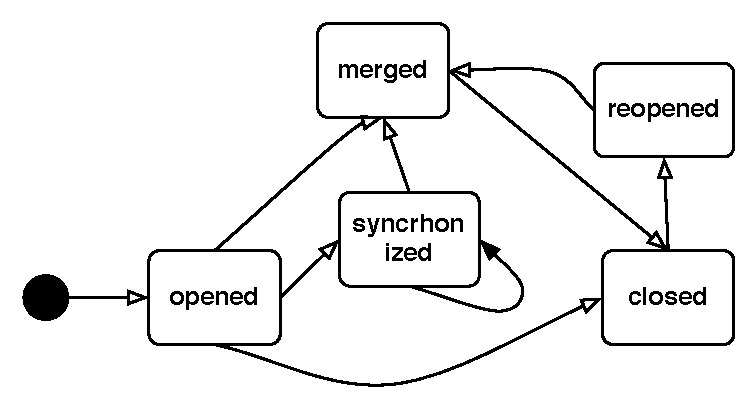
\includegraphics[scale=0.5]{pr-state-machine.pdf}
  \end{center}
  \caption{States into which a Github pull request can be into}
  \label{fig:state}
\end{figure}

By default, pull requests are submitted to the base repository for review.
Reviews can either target the pull as whole or the individual commits,
thereby resembling a code review. 
Even though any Github user can participate to the
review process, usually it is project community members that do so:
only 0.011\% of pull request comments come from users that have not
committed to the project repository.
Pull requests receive comments quite frequently: on average, each pull
request receives 12 (quantiles: 5\%: 2, 95\%: 35) discussion comments.

As a result of the discussion, pull requests can be updated with new commits or
be closed as redundant or uninteresting. To merge a pull request, a user must
be part of the main project team. The versatility of the Git tool suite enables
pull requests to be merged in various ways, presented below ordered by
the amount of preservation of the original source code properties:

\begin{description}

  \item[Through Github facilities] Github can automatically verify whether a
    pull request can be merged without conflicts to the base repository. When a
    merge is requested, Github will automatically apply the commits in the pull
    request and record the merge event. All authorship and history information
    is maintained in the merged commits.

  \item[Git merge] When a pull request cannot be applied cleanly or when
    project-related policies do not permit automatic merging, a pull request
    can be merged using plain Git utilities, using the following
    techniques: 

    \begin{itemize}

      \item \emph{Branch merging:} The remote branch containing the pull
        request commits is added as a source to a local repository. The remote 
        branch is merged to a local upstream branch, which is then pushed to
        the central repository or published for further pulling by other
        developers. Both history and authorship information are maintained,
        but Github cannot detect the merge in order to record a merge. 

      \item \emph{Cherry-picking:} Instead of merging all commits, the merger
        picks specific commits from the remote branch, which then applies to the
        upstream branch. The commit unique identifier changes, so exact history
        cannot be maintained, but authorship is preserved.
    
    \end{itemize}

    A technique that complements both of the above is \emph{commit
    squashing}: when the full history is not of interest to the project,
    several consecutive commits are merged into a single one on the pull request
    branch, which can them be merged or cherry-picked to the upstream branch. In
    this case, the author of the commit is different from the person that
    applied the commit.

  \item [Committing the patch] Through this technique, the merger creates a
    textual difference between the upstream and the pull request branch, which
    then applies to the upstream branch. Both history and authorship information
    is lost.

\end{description}

Pull requests are enabled by default on all repositories opened on Github.  From
the set of original repositories as described above, 88.000 (or 14\%) received
at least one pull request in 2012.  While the mean number of pull requests per
project is relatively low at 6.5 (percentiles: 5\%: 2, 95\%: 19), the
distribution of pull requests in projects is highly skewed, as shown in
Figure~\ref{fig:prfreq}.  A few large projects (such as the Homebrew package
manager and the Ruby on Rails web application framework) receive the vast
majority of pull requests. From the pull requests that have been opened in
2012, 66,42\% have been merged, thereby indicating that pull requests in
principle can work as a medium for obtaining external contributions.  Moreover,
even though one might expect that it is the well known projects that receive
most pull requests, this is not supported by our data: the Kendall rank
correlation between the number of watchers of a project and the number of pull
requests it has received is 0.32 ($p < 0.001, n = 63335$).

\begin{figure}
  \begin{center}
    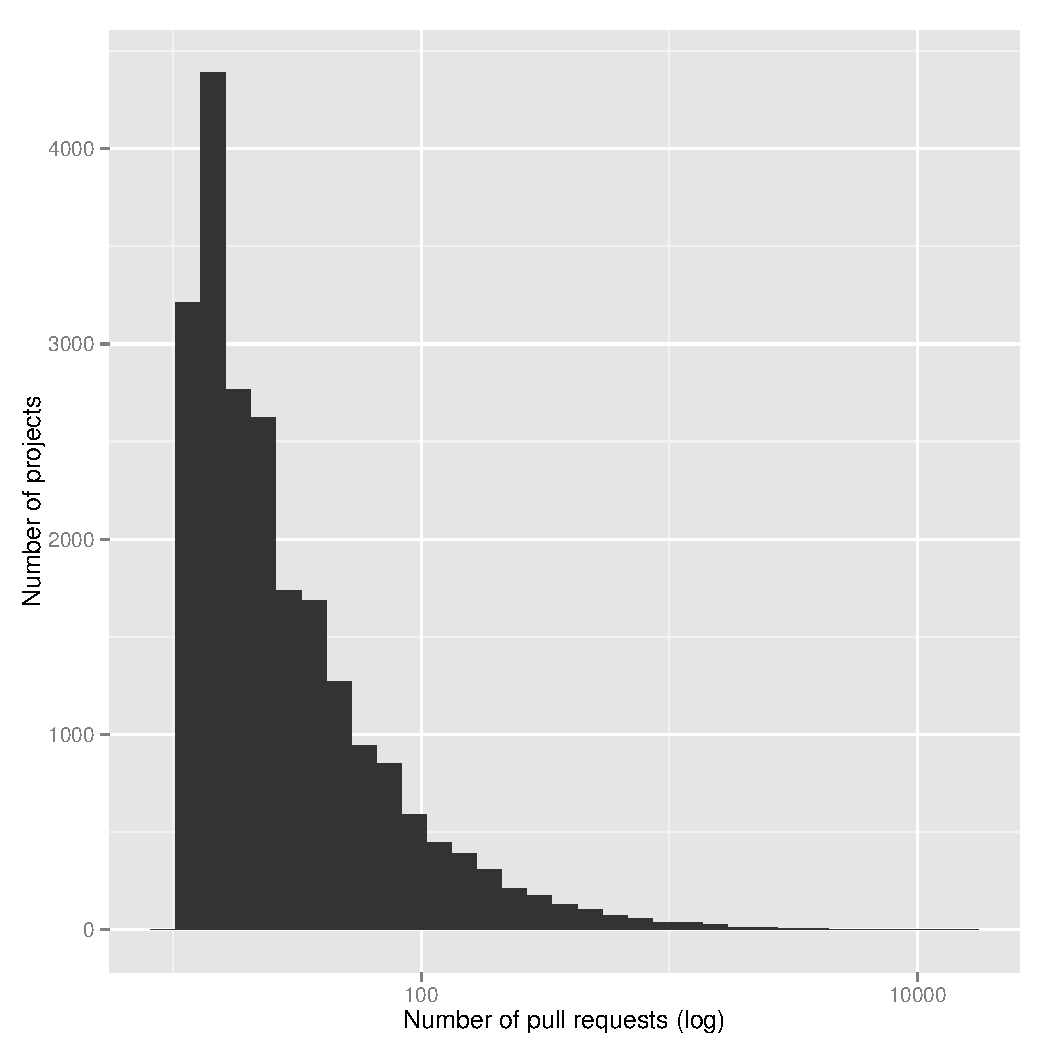
\includegraphics[scale=0.4]{pull-req-freq}
  \end{center}
  \caption{Histogram of pull request frequencies for projects with more than
  10 pull requests.}
  \label{fig:prfreq}
\end{figure}

Issues and pull requests are dual on Github; for each pull request, an issue is
opened automatically. Commits can also be attached to issues to convert them to
pull requests (albeit with external tools). This duality enables project
administrators to treat pull requests as work items, which can be managed using
the same facilities used for issues. Across projects that received pull
requests in 2012, 35\% also received a bug report (not pull-request based) 
on the Github issue tracker, indicating a strong use of Github's collaboration
facilities by both the project and the project community.

Pull requests are initially 
As can be seen in Figure~\ref{fig:before-after-pr}, on certain
long lived projects, the introduction of pull requests has significantly
increased the number of contributors per month. To investigate whether the
introduction of pull requests had a measurable effect on projects that used
them, we calculated the mean number of active developers per month for a period
of 12 months before and after the introduction of pull requests. We filtered out
projects that begun using pull requests only after September 2011 and those
whose average number of developers is less than two (indicating self-submission
and acceptance of pull requests). We performed a paired Mann-Whitney test
across the means for each project, which indicated a statistically significant
difference ($n = 362, V = 56690, p < 0.001$). We also calculated the effect size
using Cliff's $\delta = 0.42$. This indicates a significant increase in the
mean number of developers per month after the introduction of pull requests,
even though this does not necessarily mean that pull requests are indeed the
reason.

\begin{figure}
  \begin{center}
    
\includegraphics[scale=0.5]{num-commiters-after-pr}
  \end{center}
  \caption{Number of committers before and after the introduction of pull
  requests by Github. The lines are smoothed using the local polynomial
  regression fitting method, to account for monthly fluctuations.}
  \label{fig:before-after-pr}
\end{figure}

\section{Data Preparation}

To answer the research questions, we used data from the GHTorrent dataset.
Github offers two types of data through its {\sc api}; a streaming data flow
listing events, such as forking or creating pull requests, happening on
repositories and a static view of entity states. To obtain references to the
roots of the static view entities, the GHTorrent project follows the event
stream. From there, it applies a recursive dependency-based parsing approach to
yield all data offered through the {\sc api}. The GHTorrent dataset covers a
broad range of development activities on Github, including pull requests and
issues. Up to Feb 2013, more than a million pull requests from more that a
hundred thousand projects have been collected.

\subsection{Case Selection}
\label{sec:caseselection}
In the previous section, we defined pull based development, and presented an
overview of how it works across all projects on Github. While an overview of
the activity in 2012 can be safely extracted from the dataset, several
limitations would not allow us to apply our detailed analysis across all
projects. Specifically, due to the incremental nature of the GHTorrent dataset
collection, only data that are linked from events (and their dependencies) are
being collected. Projects worth analyzing have a history longer than a year, so
it is important to retrieve all information available during the project's
life. To make the data collection, and subsequent analysis, practical, we
restricted our input data to two datasets, a \textsf{handpicked} and a
\textsf{random} one. Both datasets contain 50 projects of different sizes
each. To build the datasets, we used the following criteria when selecting
projects to include:

\begin{itemize}

  \item Projects should have more than 10 pull requests in total. This is
    to filter out toy projects. 

  \item Projects should include tests. To measure the effect of testing on pull
    request acceptance, we could only use projects that include tests which we
    could measure reliably. For that, we exploited the convention-based project
    layout in the Ruby (Gem), Java and Scala (both Maven) language ecosystems,
    so our project selection was limited to those languages. 

  \item Projects should have a committer count larger than the main team member
    count, to ensure that the project is open to external contributions and that
    pull requests are indeed used by developers outside the project.

\end{itemize}

The \textsf{handpicked} dataset was created by browsing Github's top projects
per language for projects that met the criteria. The \textsf{random} dataset
was created by performing a random selection in the GHTorrent database. In
cases were the randomly selected projects did not match the criteria (existence
of tests could not be evaluated automatically) or overlapped with the
\textsf{handpicked} dataset, the non-matching projects where replaced with
other random projects. 

After selection, the datasets where merged, the full history (including pull
requests, issues and commits) of the included projects was downloaded and
features were extracted through GHTorrent database queries and analysis of each
project's Git directory. To compensate for pull requests that are merged using
Git facilities, we examined whether at least one of the commits associated with
the pull request appears in the list of commits of the target project. In case
commit squashing or patch-based merge has occurred, the merge could not be
detected, and therefore the pull request was marked as unmerged. We
investigated cases where the pull request merge ratio was significantly less
(in some cases, as small as 10\%) than the one we calculated across Github
(66\%), as this might mean that non-authorship preserving merges occurred. We
filtered out 13 projects, which we did not replace. 

The final dataset consisted of 87 projects (42 Ruby, 34 Java, 11 Scala)
and 35,466 data points (pull requests).

\subsection{Feature Selection}

For each pull request, we collected the features indicated in
Table~\ref{tab:features}.  The feature selection was based on prior work in the
areas of patch submission and
acceptance~\cite{Nagap05,Bird07a,Weiss08,Jeong09}, bug triaging~\cite{} and
also on the semi-structured interviews of Github developers in Pham et
al.~\cite{Pham13}. All features that contain a temporal dimension in their
calculation (e.g.  \texttt{team\_size} or \texttt{commits\_on\_files\_touched})
are calculated in a time window of $t - 3$ months, where $t$ is the time the
pull request has been submitted.  The presented list of 13 features has been
already pre-processed; the initial selection included more a more fine grained
list of 23 features, which we trimmed through cross-correlation analysis. For
example, we removed the features \texttt{asserts\_per\_kloc} and
\texttt{test\_cases\_per\_kloc} as they where very strongly correlated ($\rho >
0.92$) with the included \texttt{test\_lines\_per\_kloc} feature.  The features
are split among three categories:

\begin{description}

  \item[Pull request impact] features attempt to quantify the impact of the
    pull request on the affected code base. When examining external code
    contributions, the size of the patch is affecting both acceptance and
    acceptance time~\cite{Weiss08}. There are various metrics to determine the
    size of a patch that have been used by researchers: code
    churn~\cite{Nagap05, Ratzi07}, changed files~\cite{Nagap05} and number of
    commits.\todo{Refs} In the particular case of pull requests, developers
    reported that tests in a pull request increases their confidence to merge
    it~\cite{Pham13}. To investigate this, we split the churn feature to two
    features, namely \texttt{src\_churn} and \texttt{test\_churn}.

  \item[Project characteristics] features quantify how receptive to pull
    requests is the project at the time the pull request was initiated.
    If the project's process is open to external contributions, then
    we expect to see an increased ratio of external contributors over
    team members. The project's size may be a detrimental
    factor to the speed of processing a pull request, as its impact maybe
    more difficult to assess~\todo{ref}.
    Also, incoming changes tend to cluster over time (the ``Yesterday's
    weather'' change pattern~\cite{Girba04}), so it natural to assume
    that pull requests affecting a part of the system that is under
    active development will be more likely to merge.
    Testing plays a role in speed of processing; according
    to~\cite{Pham13}, projects struggling with constant flux of contributors 
    use testing, manual or preferably automated, a safety net to handle
    contributions from unknown developers.

  \item[Developer] based features quantify the influence that the person that
    created the pull request has on the decision to merge a pull request and
    the time to process it. In particular, the developer that created the patch
    has been shown to influence the patch acceptance decision~\cite{Jeong09}. To
    abstract the results across projects with different developers, we also
    include features that quantify the developer's track record, namely then
    number of previous pull requests and their acceptance rate; the former has
    been indicated as a strong indicator of pull request quality~\cite{Pham13}.
    Finally,Bird et al.~\cite{Bird07}, presented evidence that social
    reputation has an impact on whether a pull request; while the number of
    followers on Github would be an interesting proxy for reputation, technical
    details in the Github {\sc api} implementation did not allow us to calculate
    it reliably.~\footnote{The Github {\sc api} does not report a timestamp on
    when a user followed another user, so it is impossible to know how many
    followers a user had at a time instance.}

\end{description}

To check whether the selected features are independent enough, and therefore
have strong explanatory power, we conducted a pair-wise correlation analysis
using the Spearman rank correlation ($\rho$) metric across all features.  The
result can be seen in Figure~\ref{fig:crosscor}. In general, very few features
are correlated at a value $\rho > 0.2$, while only two, \texttt{src\_churn} and
\texttt{files\_changed}, are strongly correlated at $\rho = 0.71$. While the
correlation is strong, it is not definite and therefore we do not remove either
feature from the dataset. All results are statistically significant ($n =
35,466, p < 0.001$).

\begin{table*}
  \begin{small}
  \centering
  \begin{tabular}{rp{40em}}
    \hline
    \bf{Feature} & \bf{Description and Justification}\\
    \hline
    \multicolumn{2}{l}{\bf{Pull Request Impact}}\\
    
    \texttt{num\_commits} & Number of commits in the pull request. A bigger
    pull request will be slower to examine and therefore to merge.\\
    
    \texttt{src\_churn} & Number of lines changed (added + deleted) by the pull
    request. The more lines changed, the longer a pull request will take to be
    reviewed.\\

    \texttt{test\_churn} & Number of test lines changed in the pull request. Pull requests
    that include tests should be easier to merge, as testing would increase
    confidence for the merger.\\
    
    \texttt{files\_changed} & Number of files touched by the pull request. An
    indication of the impact of the pull request.\\
    
    \texttt{num\_comments} & The total number of comments (discussion and code
    review). More pull code review comments may indicate a rigorous process,
    therefore slowing down acceptance.\\

    \multicolumn{2}{l}{\bf{Project Characteristics}}\\
    
    \texttt{sloc} & Executable lines of code at pull request merge time. The
    bigger the project, the more difficult would be to assess the impact of
    a pull request. \\

    \texttt{team\_size} & Number of active core team members during the last
    3 months prior the pull request creation. A big team will be faster to process a
    pull request as each team member will have less work load to handle and
    will be more specialized.\\

    \texttt{perc\_external\_contribs} & The ratio of commits from external
    members over core team members in the last 3 months prior to pull request
    creation. A higher ratio indicates a more open
    process, which may lead to more accepted pull requests.\\

    \texttt{commits\_on\_files\_touched} & Number of total commits on files
    touched by the pull request 3 months before the pull request creation time.
    If the pull request touches files in a hotspot, it will be merged faster.\\
 
    \texttt{tests\_per\_1000\_lines} & A proxy for the project's test
    coverage. The more well tested a project is, the faster a pull request
    could be merged, as applying it and testing its impact would be faster. \\

    \multicolumn{2}{l}{\bf{Developer}}\\
    
    \texttt{prev\_pullreqs} & Number of pull requests submitted by a specific
    developer, prior to the examined pull request. The more pull requests, the
    better the developer is known to the project.\\

    \texttt{requester\_succ\_rate} & The percentage of the developer's pull requests that have been merged up to the creation of the examined pull
    request. A high success rate indicates a developer trusted by the project.\\

    \texttt{main\_team\_member} & Whether the developer belongs to the
    main repository team. Pull requests from main team members should be
    faster to accept and merge due to increased confidence.\\
    \hline
  \end{tabular}
  \caption{Selected features and justification}
  \label{tab:features}
  \end{small}
\end{table*}

%\begin{table*} \centering 
%  \caption{Descriptive statistics of the examined dataset} 
%\footnotesize 
%\begin{tabular}{@{\extracolsep{5pt}}l c c c c c c } 
%\\[-1.8ex]\hline 
%\hline \\[-1.8ex] 
%Statistic & \multicolumn{1}{c}{\textit{N}} & \multicolumn{1}{c}{\textit{Mean}} & \multicolumn{1}{c}{\textit{St. Dev.}} & \multicolumn{1}{c}{\textit{Min}} & \multicolumn{1}{c}{\textit{Median}} & \multicolumn{1}{c}{\textit{Max}} \\ 
%\hline \\[-1.8ex] 
%lifetime\_minutes & 46,093 & 15,541.840 & 57,947.680 & 0 & 806 & 1,211,940 \\ 
%mergetime\_minutes & 28,393 & 6,840.924 & 29,358.100 & 0 & 363 & 809,307 \\ 
%team\_size & 46,093 & 30.494 & 38.646 & 0 & 14 & 178 \\ 
%num\_commits & 46,093 & 4.528 & 21.276 & 0 & 1 & 1,379 \\ 
%files\_changed & 46,093 & 42.657 & 341.695 & 0 & 3 & 18,450 \\ 
%perc\_external\_contribs & 46,093 & 46.042 & 27.256 & 0 & 45 & 100 \\ 
%sloc & 46,093 & 97,443.830 & 139,809.200 & 26 & 43,867 & 730,109 \\ 
%src\_churn & 46,093 & 631.171 & 4,577.060 & 0 & 13 & 301,094 \\ 
%test\_churn & 46,093 & 171.579 & 1,360.882 & 0 & 0 & 85,535 \\ 
%commits\_on\_files\_touched & 46,093 & 92.025 & 675.993 & 0 & 1 & 35,806 \\ 
%test\_lines\_per\_1000\_lines & 46,093 & 804.886 & 827.935 & 0.000 & 568.358 & 5,357.608 \\ 
%prev\_pullreqs & 46,093 & 35.299 & 56.809 & 0 & 10 & 405 \\ 
%requester\_succ\_rate & 46,093 & 0.479 & 0.407 & 0.000 & 0.550 & 1.000 \\ 
%\hline \\[-1.8ex] 
%\normalsize 
%\end{tabular} 
%\end{table*} 

\begin{figure}
  \begin{center}
    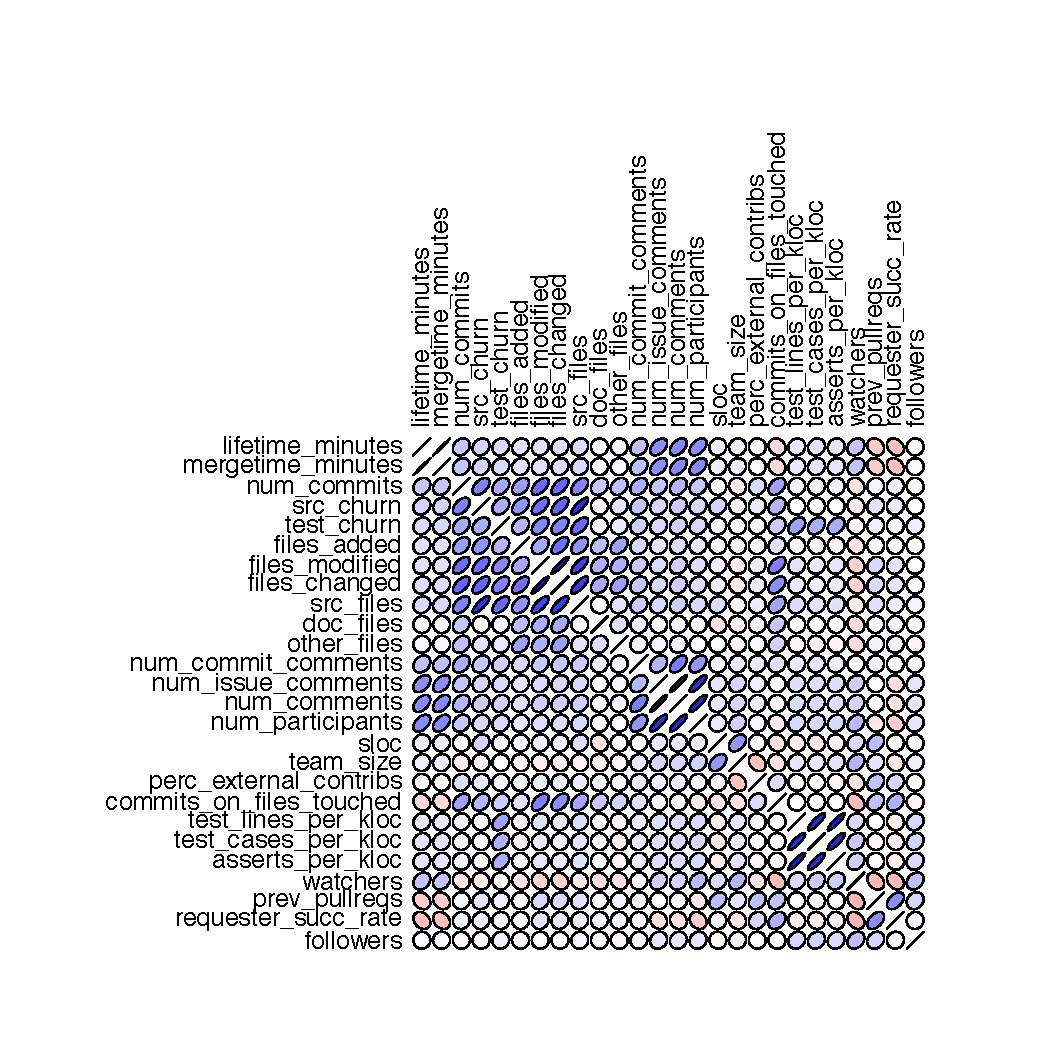
\includegraphics[scale=0.6]{cross-cor.pdf}
  \end{center}
  \caption{Cross correlation matrix (Spearman) for selected features. The more elliptical a point is, the strongest the correlation. A right slant indicates
  a positive correlation.}
  \label{fig:crosscor}
\end{figure}

\subsection{Pull Request Characteristics}

In this section, we analyse the 

\paragraph*{Lifetime of pull requests}

After being submitted, pull requests can be in two states: merged or closed
(and therefore not-merged).~\footnote{Intermediate states shown in
Figure~\ref{fig:state} are added by the Github pull request handling process.} 
Figure~\ref{fig:perc-merged} shows the distribution of merged vs unmerged
pull requests across projects in our dataset. What we can see is that
in most projects, most pull requests (75,5\%, mean: 74.5\%) are getting
merged. This result is slightly higher than the overall we calculated for
Github, but this can be attributed to the fact that the dataset was cleaned
from projects for which we could not detect merges accurately. 
The merged pull request percentage is almost normally distributed among projects (Shapiro-Wilkes test: $n = 82, p > 0.06$) with a standard deviation $\sigma = 14.68$. 

For merged pull requests, an important property is the time required to process
and merge them. The time to merge distribution is highly skewed
(Figure~\ref{fig:pull-req-patch} displays a log transformed histogram), with
the great majority of merges happening very fast. Measured in days, 95\% of the
pull requests are merged in 19, 90\% in 8 and 80\% in only 2.8 days. An
interesting observation is that there are many (8525 or 30\%) pull requests
which are merged in under one hour; the majority of such pull requests (60\%)
come from core team members, while their source code churn is significantly
lower than that of the remaining pull requests.
Based on this observation, a question that emerges is whether the pull
requests originating from main team members are treated faster that those
from external contributors. To answer it, we performed an unpaired Mann-Witney
test among the times to merge pull requests from each group. The result
is that while the two groups differ in a statistically significant manner ($n1 = 14316, n2 = 12463, p < 0.001$), the apparent difference
is very small (Cliff's $\delta: -0.11$, see also Figure~\ref{fig:lifetime-boxplot}). This means that merged
pull requests received no special treatment, even if they came from core
team members.

On a per project basis, if we calculate the mean time to merge a pull request,
we see that in the majority of projects (72\%), the time to merge a pull
request is less than 7 days. The mean time to merge a pull request per project
is not directly correlated to the project's size ($\rho = -0.23$) nor to the
project's test coverage ($\rho = 0.34$) Moreover, projects are not getting
faster by processing more pull requests; the correlation between the average
time to merge and the number of pull requests is very weak ($\rho = -0.33, n =
82, p < 0.01$).

\begin{figure*}
\centering
\subfigure[Percentage of pull requests that have been merged per project.
Project names are omitted for clarity.]{
  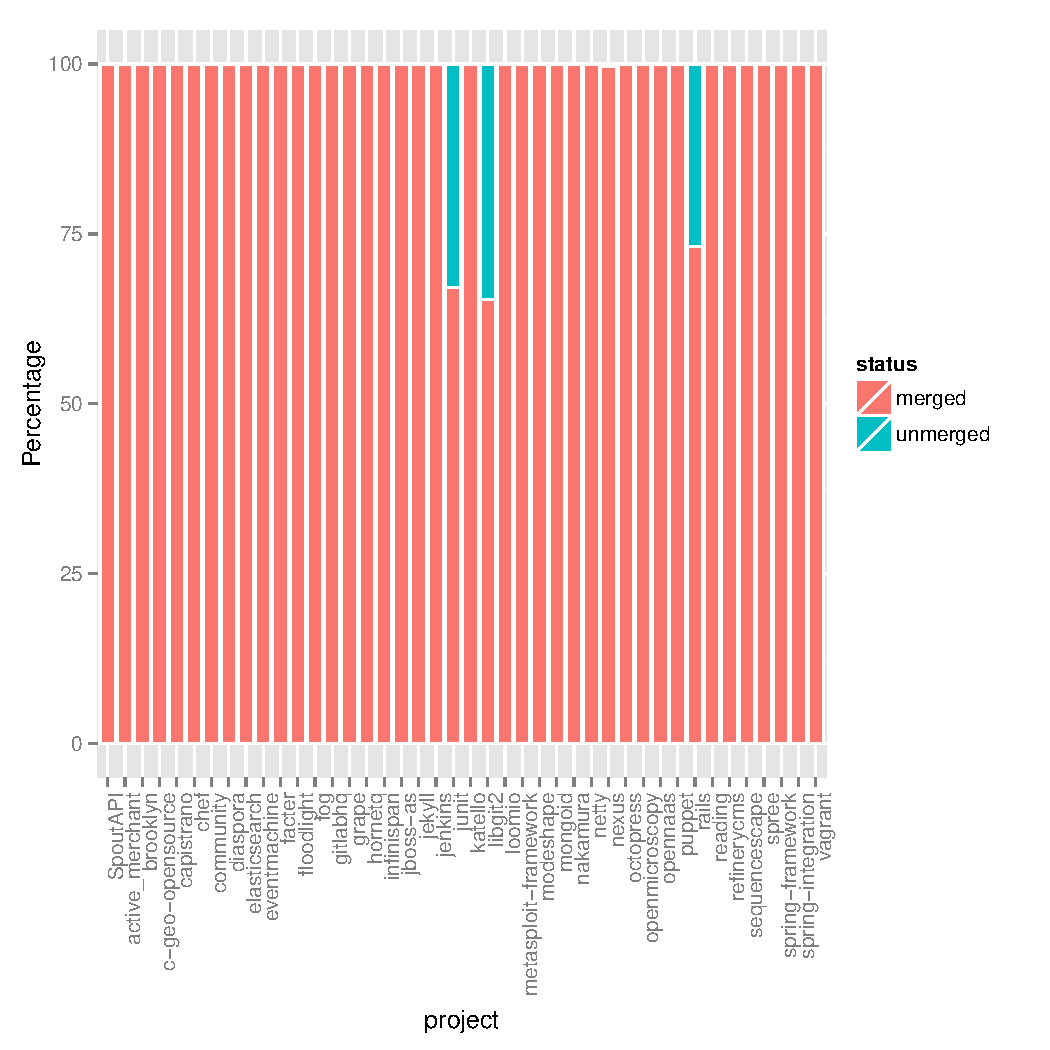
\includegraphics[scale=0.3]{perc-merged.pdf} 
  \label{fig:perc-merged}
}
\subfigure[Time to merge pull requests]{
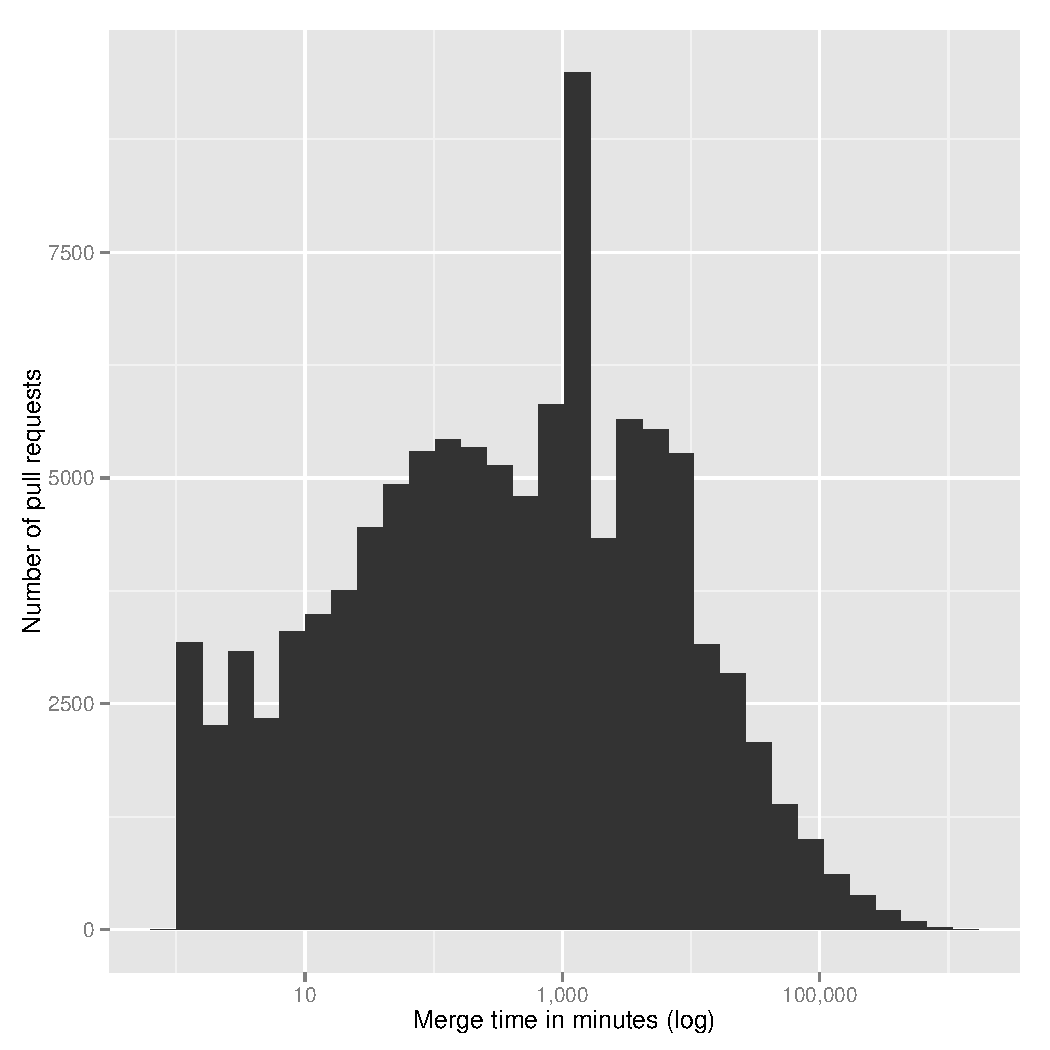
\includegraphics[scale=0.3]{pr-lifetime-hist.pdf}
\label{fig:pull-req-merge-time}
}
\subfigure[Time to merge pull requests for internal vs external team members.]{
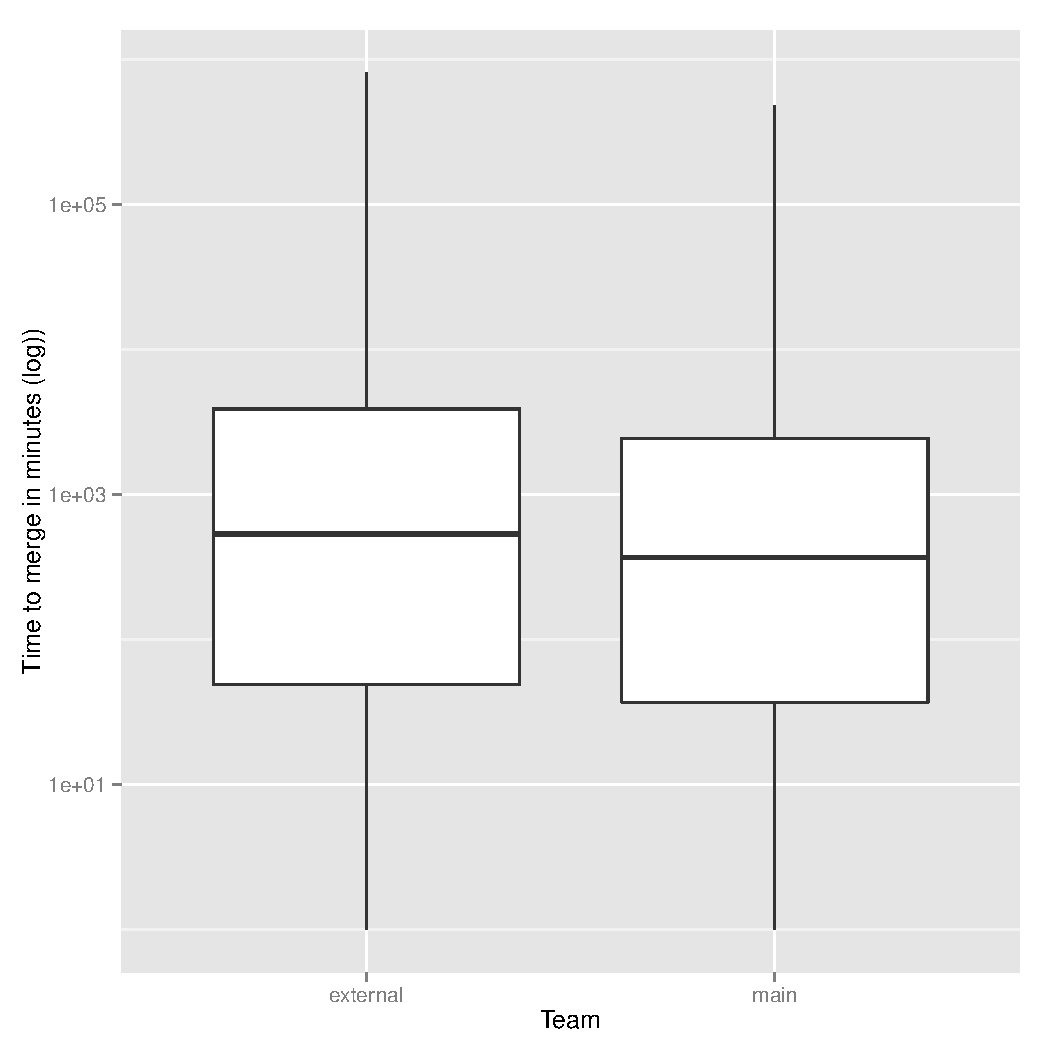
\includegraphics[scale=0.3]{merge-internal-external.pdf}
\label{fig:lifetime-boxplot}
}
\subfigure[Size of pull request patch]{
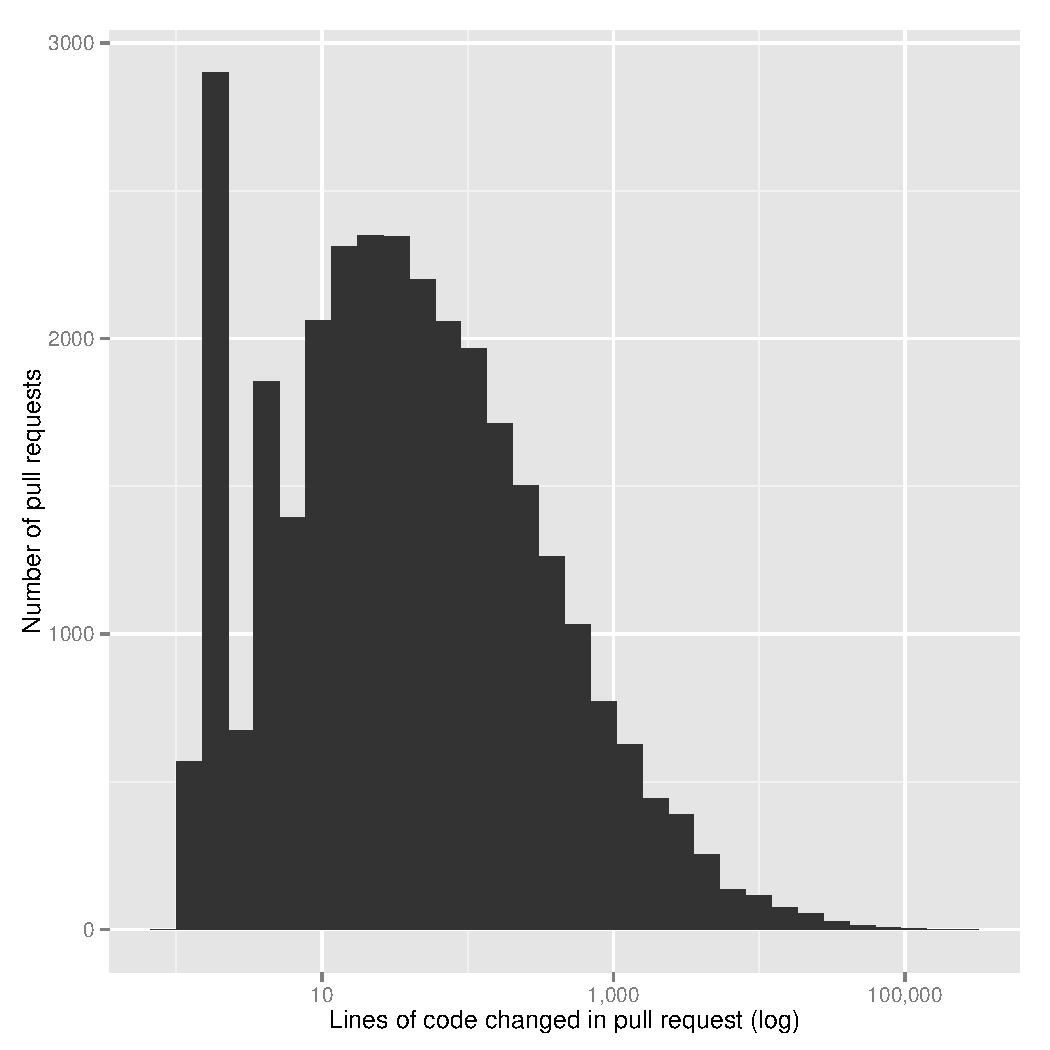
\includegraphics[scale=0.3]{pr-size-hist.pdf}
\label{fig:pull-req-patch}
}
\subfigure[Number of files changed by pull request]{
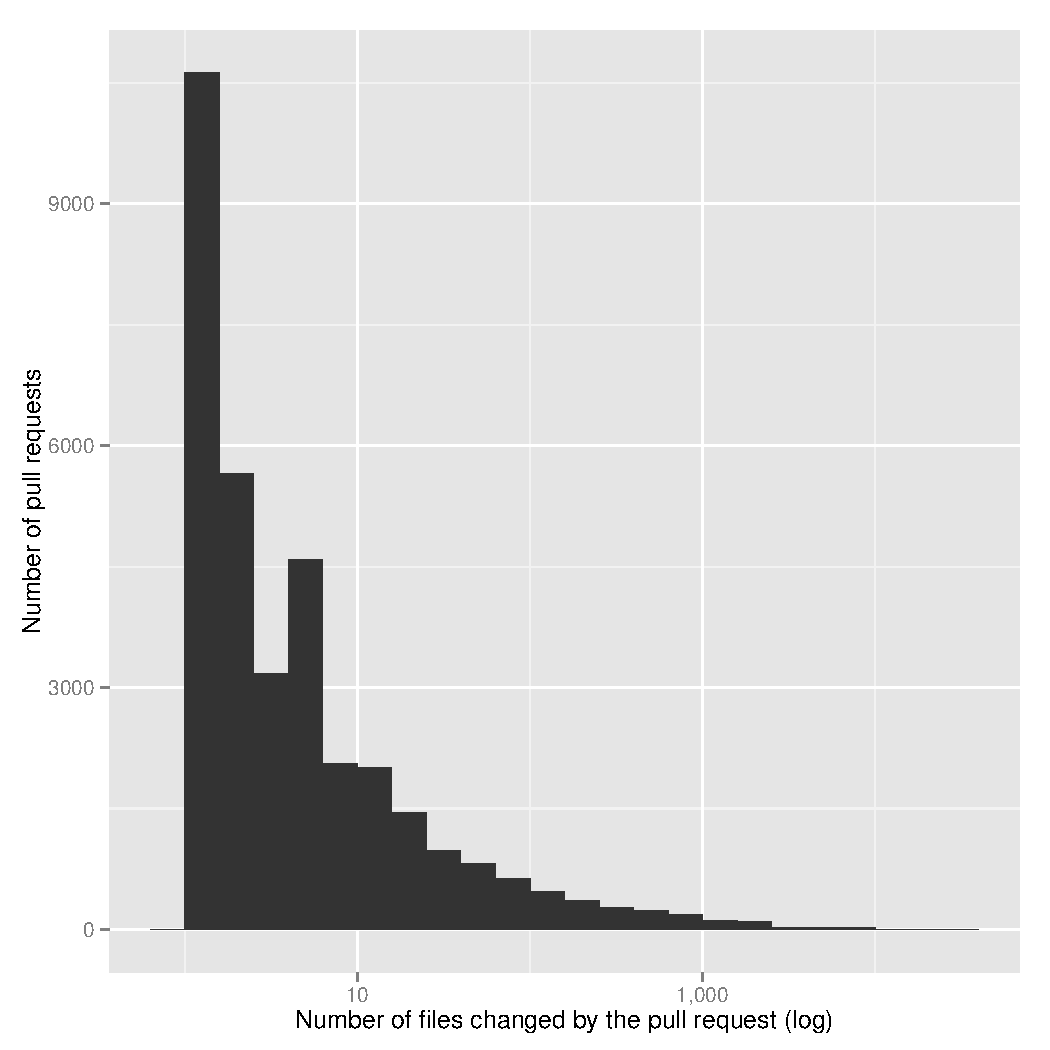
\includegraphics[scale=0.3]{pr-size-files-changed-hist.pdf}
\label{fig:pull-req-files}
}
\subfigure[Number of comments]{
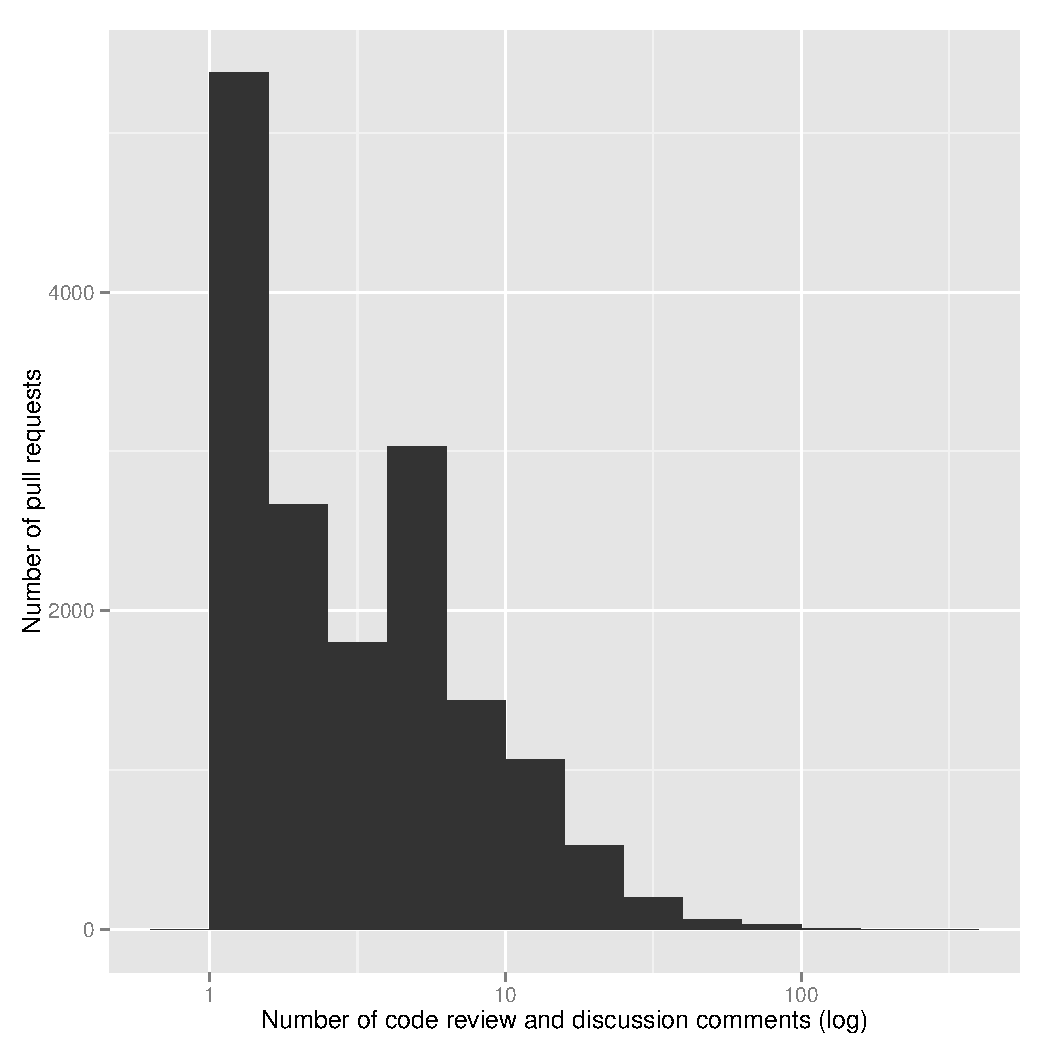
\includegraphics[scale=0.3]{pr-num-comments-hist.pdf}
\label{fig:pull-num-comments}
}
\caption{Dataset characteristics}
\end{figure*}

\paragraph*{Sizes of pull requests}

%Pull requests are essentially an organized way to submit patches.
A pull request bundles together a set of commits; the number of 
commits on a pull request is generally less than 10 (95\% percentile 11,
90\% percentile 6, 80\% percentile 3). Similarly, the number of 
files that have changed 



Except from the project's source code, pull requests also modify test
code. In our sample, 33\% of the pull requests included modifications
in test code, while 4\% modified test code exclusively. Of those
pull requests, 72\% was merged; this result is inline with the findings by
Pham et al.~\cite{Pham13} where interviewed developers identified 
the presence of tests as a major factor for the acceptance of pull requests.

\paragraph*{Discussion and Code review}

Once a pull request has been submitted, it is open for discussion until
it is merged or closed. The discussion is usually brief: 95\% of pull
requests receive 10 comments or less (80\% less than 4 comments). 


\section{Acceptance and Processing Speed}
\label{sec:accrej}

To answer both our research questions, we conducted a set of prediction
experiments using the dataset presented in the previous section.
The purpose of the experiments was not to create accurate prediction
models, but rather to evaluate the importance of each feature
in the pull request handling process. Therefore, in our discussion, 
we skip some details on the configuration of the various
prediction algorithms we used.

Prior to running the classification algorithms, we labeled each data point with
a binary attribute; in the case of the merge decision problem, the attribute
signified whether the pull request has been merged. For the merge time problem,
we first filtered out pull requests that have not been merged and then split
the remaining data points in two bins, slow and fast, using the mean time to
merge (6613 minutes, as calculated above) as the split point. The dataset
sizes were 35,466 and 26,779 points for the merge decision and merge time
classification task, respectively.

At a high level, the process to retrieve the dominant features for both
problems consisted of two steps: i) we run each dataset through 4 well known
classification algorithms, namely Random Forests (\texttt{randomforest}),
Support Vector Machines (\texttt{svm}), Binary Logistic Regression
(\texttt{binlogregr}) and Na\"ive Bayes (\texttt{naivebayes}), ii) we select
the best classifier and apply a classifier specific process to extract the
feature importance. In all cases, we used the full set of features and
trained the classifier against the applicable binary attribute.

To select the appropriate classification algorithm, we run a 10-fold random
selection cross-validation and aggregated the mean values for each
classification metric. At each iteration, the algorithm would randomly sample
10,000 data points from the whole dataset, train a classifier with 90\% percent
of the input and use it to predict the remaining 10\%. The 10-fold run results
also allowed us to evaluate the metric stability across runs. To evaluate the
classification performance, we used the Accuracy ({\sc acc}) and Area Under the
receiver operating characteristic Curve ({\sc auc}) metrics. We chose those as
opposed to the more popular Precision ({\sc prec}) and Recall ({\sc rec}) ones,
following advice in reference~\cite{Lessm08}. We did not perform any additional
tuning to the classification algorithms. The implementations of the R
statistics language were used for running the experiments.

\begin{table}
  \centering
  \begin{tabular}{lcccc}
    \hline
    {\bf classifier} & {\sc auc} & {\sc acc} & {\sc prec} & {\sc rec} \\
    \hline
    \multicolumn{4}{l}{\textsf{merge time task}($n = 26,779$)} \\
    binlogregr    & 0.60 & 0.55 & 0.56 & 0.57  \\
    naivebayes    & 0.58 & 0.54 & 0.54 & 0.57  \\
    randomforest  & 0.73 & 0.61 & 0.65 & 0.70  \\
    svm           & 0.54 & 0.49 & 0.45 & 0.45  \\
    \hline
    \multicolumn{4}{l}{\textsf{merge decision task}($n = 35,466$)} \\
    binlogregr    & 0.73 & 0.63 & 0.87 & 0.58  \\
    naivebayes    & 0.69 & 0.61 & 0.85 & 0.57  \\
    randomforest  & 0.94 & 0.87 & 0.93 & 0.93  \\
    svm           & 0.52 & 0.48 & 0.72 & 0.48  \\
    \hline
  \end{tabular}
  \caption{Classifier performance for the merge decision and merge time
  classification tasks. The results are means of 10-fold random selection
  cross validation (sample size 10,000), with 90\% train and 10\% test data.}
  \label{tab:classif-perf}
\end{table}

Based on the results presented in Table~\ref{tab:classif-perf},
we selected the \texttt{randomforest} classification algorithm for
both our experiments. For the \textsf{mergetime} task, \texttt{randomforest}
achieved an {\sc auc} of 0.73, with a prior probability of 50\%. For 
the \textsf{mergedecision} task, the prior probability was 74\% which
allowed the algorithm to achieve near perfect scores. In both cases,
the stability of the {\sc auc} metric across folds was good 
($\sigma_{auc-mergetime} = 0.019$, ($\sigma_{auc-mergedecision} = 0.008$).

\begin{figure*}
\centering
\subfigure {
  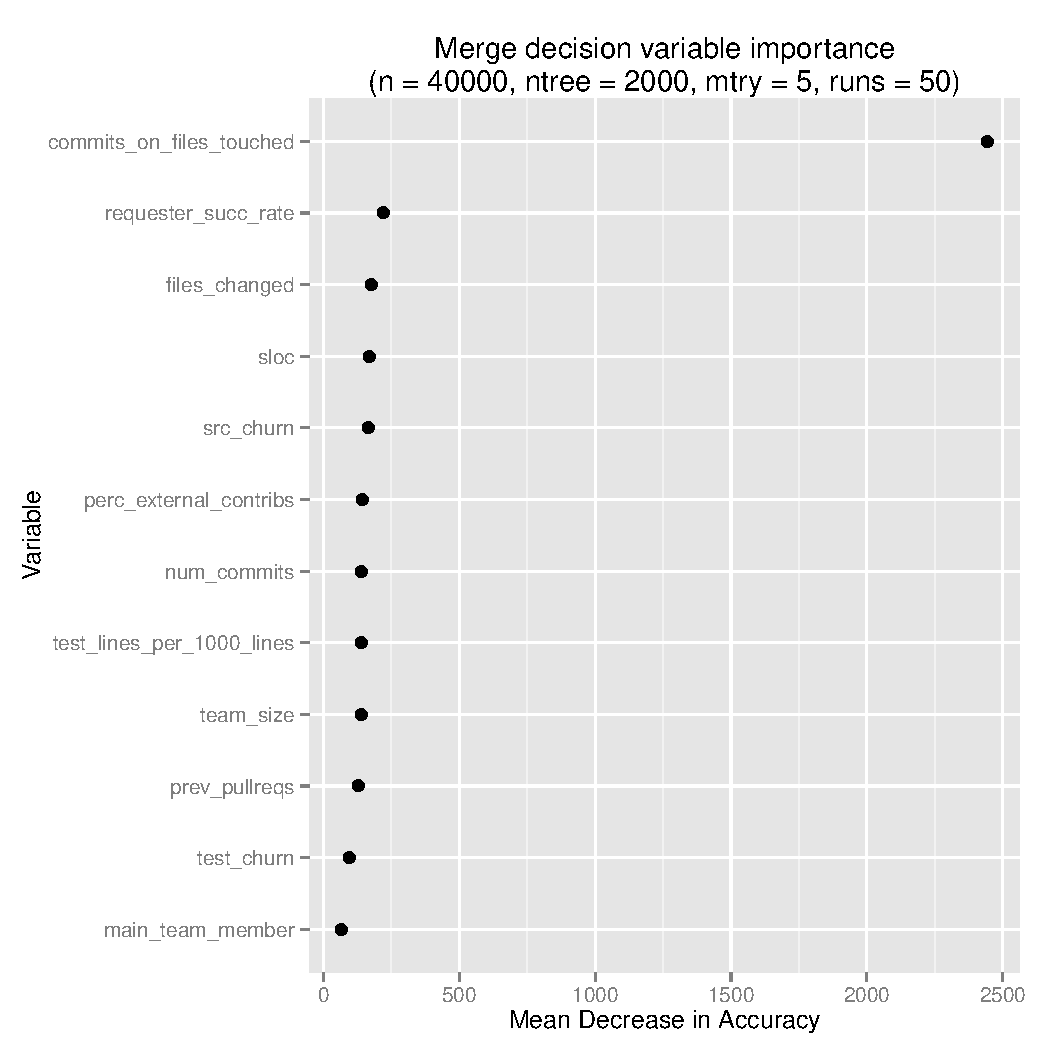
\includegraphics[scale=0.3]{varimp-merge-decision-40000-50.pdf} 
  \label{fig:varimp-merge-decision}
}
\subfigure{
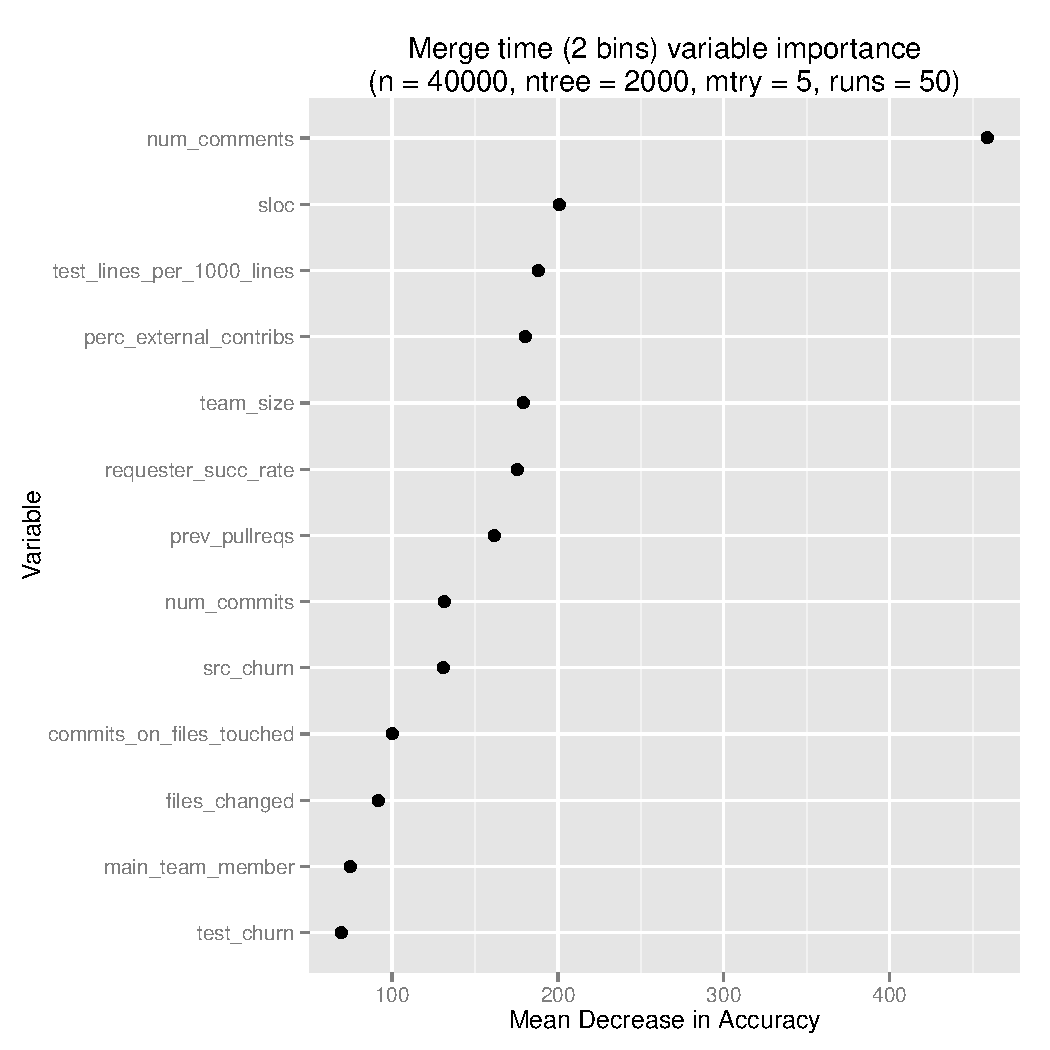
\includegraphics[scale=0.3]{varimp-merge-time-(2-bins)-40000-50.pdf}
  \label{fig:varimp-merge-time}
}
\subfigure{
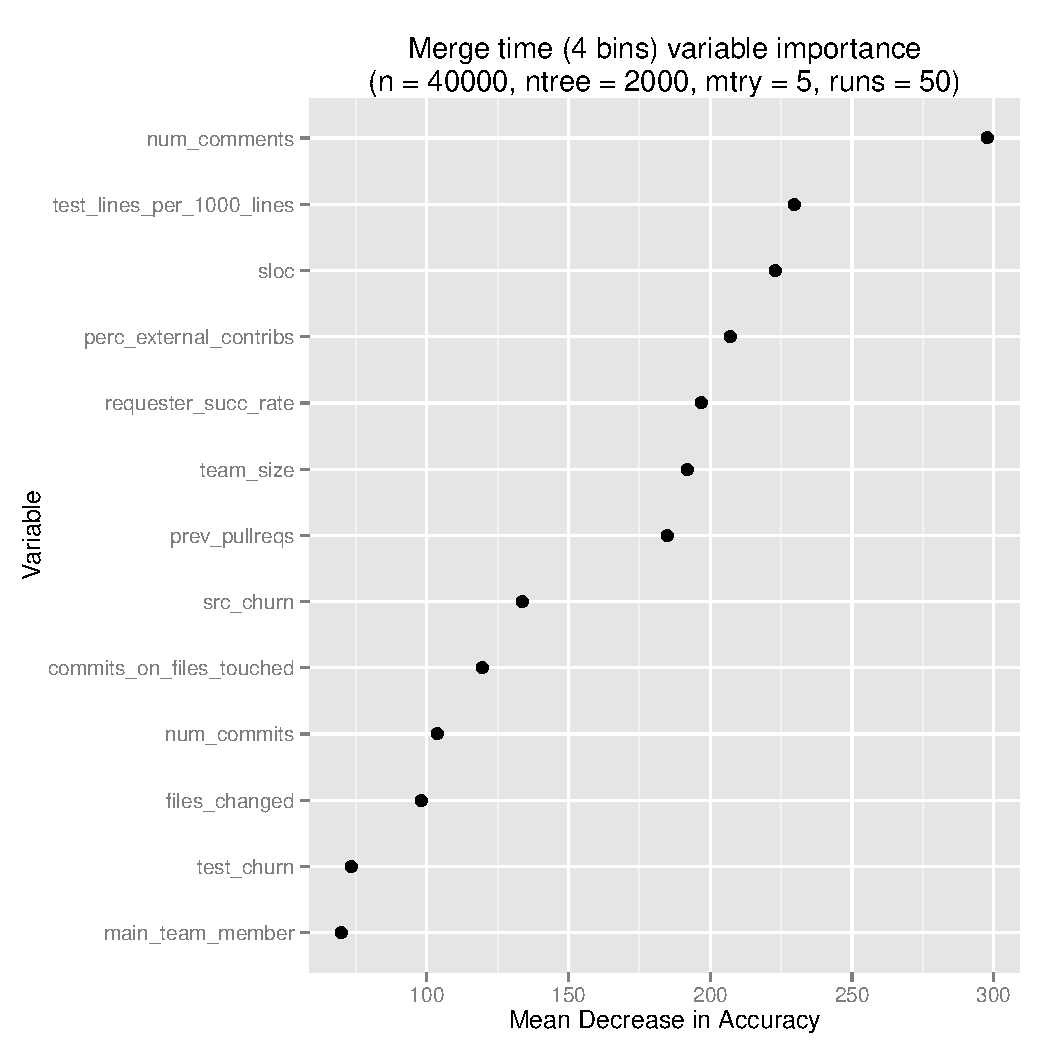
\includegraphics[scale=0.3]{varimp-merge-time-(4-bins)-40000-50.pdf}
  \label{fig:varimp-merge-time}
}
\caption{Random forest feature importance for predicting merge decision (a) and merge time (b)}
\label{fig:varimp}
\end{figure*}

To extract the features that are important for each classification task, we
used the process suggested in reference~\cite{Genue10}. Specifically, we run
the algorithm 50 times on the full dataset for each experiment, using a large
number of generated trees (2000) and trying 5 random variables per split. We
then used the mean across 50 runs of the  Mean Decrease in Accuracy metric, as
reported by the {\sc r} implementation of the random forest algorithm, to
evaluate the importance of each feature. The results can be seen in
Figure~\ref{fig:varimp}.

\paragraph{Merge Decision}

For the \textsf{mergedecision} task, the feature importance result is dominated
by the \textsf{commits\_on\_files\_touched} feature. 

\paragraph{Merge Time}

For the \textsf{mergetime} task, many variables offer similar support to the
prediction model built by the random forest algorithm. From the results, we can
conclude that the size of the project and its test coverage play a significant
role on how fast pull requests are processed. 

The results of the \textsf{mergetime} classifier may be influenced by the choice of the cutoff used for separating the pull requests to fast and slow.
To evaluate the stability of the variable importance evaluation, we conducted
a further experiment, with four bins: 


\section{Discussion}

\label{sec:discussion}

\paragraph{Development turnover} One of the promises of the pull request model
is that of fast development turnover, i.e. the time between submission of a pull
request and acceptance in the project's main repository.  In various studies of
the patch submission process in projects such as Apache and Mozilla, the
researchers found that the time to commit 50\% of the contributions to the main
project repository ranges from a few hours~\cite{Rigby08} to a less than 3
days~\cite{Weiss08, Baysal12}. Our findings show that the majority (80\%) of
pull requests are merged within 3 days, while a very significant number (30\%)
are merged within one hour. These numbers are significantly faster indicating
that pull requests are more efficient than traditional email-based patches.
What's more important is that it is project-related factors that affect the
turnover time, rather than characteristics of the pull request. This means that
it is mostly up to the project to tune its processes (notably, reviewing and
testing) for faster turnover.  

\paragraph{Attracting contributions}
In our study, we have shown that after pull requests have been introduced
by Github, several projects have seen a measurable increase in the number
of committers per month. But why is it that so? One possible explanation
is presented by Pham et al.: in reference~\cite{Pham13}, they mention
that pull requests make casual contributions straightforward through
a mechanism often referred to as ``drive-by commits''. As the
relative cost to fork a repository is negligible on Github (54\% of the
repositories are forks), it is not uncommon for developers to fork other
repositories to perform casual commits, such as fixes to spelling mistakes or
indentation issues. In addition, Github provides web based editors
for various file formats, using which any user can edit a file in another
repository; behind the scenes, Github will fork the repository and ask the user
to create a pull request to the original one. Such commits might be identified
as pull requests that contain a single commit from users that are not yet part
of the project's community. Even under this na\"ive definition, 7\% of pull
requests in 2012 can be classified as drive by commits. Moreover, 3.5\% of the
forks were created for the sole purpose of creating a drive-by commit. More
work needs to be done for the accurate definition and assessment of the
implications of drive-by commits, which we defer for future work.

\paragraph{Crowd sourcing the code review}

An important part of the contribution process to an open source project is the
review of the provided code. In reference~\cite{Rigby06}, Rigby and German
report that 80\% of the core team members are also participating in the code
reviews for patches, a number that is also in line with earlier findings by
Mockus et al.~\cite{MOCKU02}. 

ratio between core team members / code reviewers

This means that 

\paragraph{Democratizing development}
One of the findings of this work is that pull requests are not treated
differently based on their origin; both core team members and external
developers have equal chances to get their pull request accepted within
the same time boundaries. In our
opinion, this is a radical change in the way open source development
is being carried out. Before pull requests, most projects employed 
membership promotion strategies to promote interested third party
developers to the core team, where they could commit directly to the
repository. With pull requests developers can contribute to any repository, without loss of authorship information, with better chances of having
their contribution accepted. Specialized sites such as Ohloh 
and CoderWall track developer activity and help developers advertise
their expertise. We believe that the democratization of the development
effort will lead to a substantially stronger ``commons'' ecosystem; this
remains to be verified in further studies.

\subsection{Implications}

\paragraph{Contributors} Pull requests containing tests get merged more often.
If the purpose it to contribute  

\paragraph{Project Owners} Restrict discussion to absolutely necessary
Include test lines in the project, demand tests in project guidelines
Have a team size

\paragraph{Researchers} 


\subsection{Threats to validity}
Here we analyse the threats to validity of our study.

\noindent\emph{Construct validity:} Our statistical analysis uses random forests as a
way to identify and rank cross-factor importance on two response variables.
While this is a valid approach~\cite{}, we 've yet to find other studies in
empirical software engineering that follow it. Moreover, the classification
scores in the \textsf{mergetime} case are not perfect, so feature ranking may
not be exactly the same given a different dataset. Further work on validating
the models we have built on data from different data sources (e.g. manual pull
request handling in the Linux kernel) or projects in different languages on the
GHTorrent dataset.

\noindent\emph{Internal validity:}
To analyze the projects, we extracted data from i) the GHTorrent relational
database ii) The GHTorrent raw database iii) each project's Git repository.
Differences in the data abstraction afforded by each data source may
lead to different results in the following cases: 

\begin{itemize}

  \item Intra-repository merging: GHTorrent currently does not record the source
    and target branch names that are affected by a pull request. Therefore, it
    is not possible to use the heuristics presented in
    Section~\ref{sec:caseselection} to identify a merged branch (if the project
    does not use Github facilities to merge), as the source and target branches,
    and therefore their commits, are in the same repository. In those cases, we
    report the pull request as non-merged. In our dataset, 810 (or 2\% in total)
    pull requests are label as non-merged and intra-repository; some of them may
    actually be merged.

  \item Number of files and commits on touched files: The commits reported
    in a pull request also contain commits that merge branches, which the
    developer may have merged prior to performing his changes. These commits
    may contain several files not related to the pull request itself, which
    in turn usually affects our results heavily. Therefore, we decided to 
    filter out those commits.

\end{itemize}

\noindent\emph{External validity:}
In our study, we used merged data from several projects. The statistical
analysis treated all projects as equal, even though differences do exist.
For example, the larger project in our dataset, Ruby on Rails, 
has more than 8,000 pull requests while the smaller one just ~\todo{measure}.
While we believe the uniform treatment of the samples led to more robust
results in the classification experiment, variations in pull request
handling among projects with smaller core teams may be ironed out.

\subsection{On Replication}

During the execution of this study, we invested significant effort to
make it replicable.  This study has been conducted using the GHTorrent dataset
and a custom set of Ruby and R tools. We share the tools, original data sources
and extracted data files on the Github repository \texttt{gousiosg/pullreqs}.
The execution of all tools is scripted and it is possible to run it
in sequence automatically. We invite other researchers to use the tools and data
to replicate the study or create new studies based on it.

\section{Related Work}

\cite{Bird09}
\cite{Cornf10}
\cite{Dabbi12}
\cite{Bird12}
\cite{Barr12}
\cite{Buffe99}
\cite{Mens02}
\cite{Shiha12}

Global software development
\section{Conclusions and Future Work}

In this work, we only described briefly some aspects of pull request activity.
In further work, it would be interesting to investigate in depth how drive-by
commits contribute to project evolution (both in terms source code and in
terms of community) and how code proliferates among project
forks in software ecosystems.

\section*{Acknowledgements}

This work is partially supported by Marie Curie {\sc ief} 298930 -- {\sc sefunc}.

\bibliographystyle{ieeetr}
\bibliography{pullreqs}

\end{document}
